\chapter{Estado del arte}

\section{PBR}
    \subsection{Modelo f\'isico}
        Light is a complex phenomenon as it can exhibit properties of both a wave and a
        particle. As a result, different models have been created to describe its behavior.

        As texture artists, we are interested in the ray model of light as it describes the
        interaction of light and matter. Understanding how light rays interact with surface
        matter is important because our job is to create textures that describe a surface.
        The textures and materials we author interact with light in our virtual worlds. The
        more we understand how light behaves, the better our textures will look.
        
        A light ray is incident on a plane interface between two media. When a light ray
        hits a surface, one or both of the following events may occur:
        
        \begin{enumerate}
            \item
                The light ray is reflected off the surface and travels in a different direction.
                It follows the Law of Reflection, which states that the angle of reflection is equal
                to the angle of incidence (reflected light).
            \item
                The light ray passes from one medium to another in the trajectory of a straight
                line (refracted light).
        \end{enumerate}
    
        \begin{figure}[H]
            \setlength{\fboxsep}{0pt}
            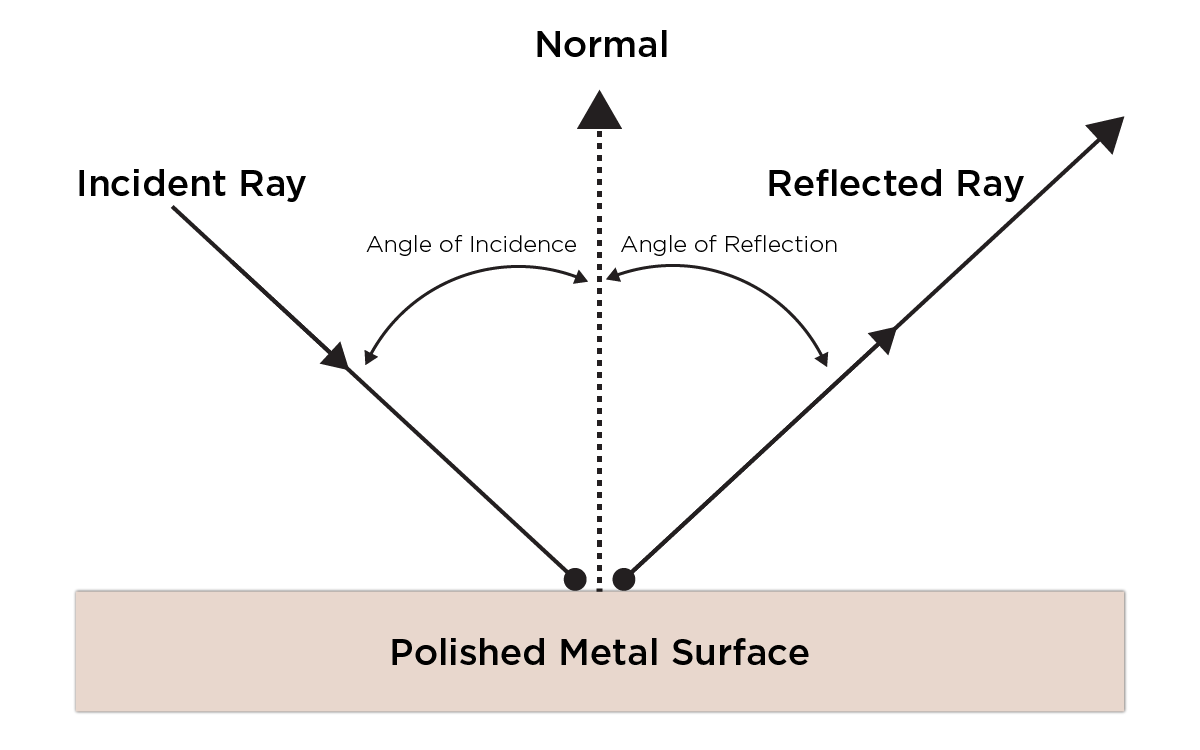
\includegraphics[width=1\linewidth]{images/substance-the_pbr_guide-incident_rays.png}
            \caption{A boat.}
            \singlespacing
        \end{figure}
        

    \subsubsection{Radiancia e irradiancia}
    \subsubsection{Reflexi\'on y refracci\'on}
    \subsubsection{Conservaci\'on de la energia}
        Energy conservation plays a vital role in physically-based rendering solutions. This
        principle states the total amount of light re-emitted by a surface (reflected and scattered
        back) is less than the total amount received. In other words, the light reflected from the
        surface will never be more intense than it was before it hit the surface. As artists, we
        don’t have to worry about controlling energy conservation. This is one of the advantages of
        PBR: energy conservation is always enforced by the shader. This is part of the physically
        based model and it allows us to focus on art rather than physics.
    \newpage

    \subsection{Representaci\'on digital}
        \subsubsection{Microfacetas}
            In theory, both diffuse and specular reflection are dependent on the surface
            irregularities where the light rays intersect with a medium. In practice however, the
            effect of roughness on diffuse reflection is less visible because of the scattering
            that occurs inside the material. As a result, the outgoing direction of the ray is
            fairly independent of surface roughness and the incident direction. The most common
            model for diffuse reflection (Lambertian) completely neglects roughness.

            In this guide, we refer to these surface irregularities as surface roughness. Surface
            irregularities can have several other names, including roughness, smoothness,
            glossiness or micro-surface, depending on the PBR workflow in use. All these terms
            describe the same aspect of a surface, which is sub-texel geometric detail.
            
            These surface irregularities are authored in the roughness or glossiness map depending
            on the workflow that is being used. A physically-based BRDF is based on the microfacet
            theory, which supposes that a surface is composed of small-scaled planar detail surfaces
            of varying orientation called microfacets. Each of these small planes reflects light in
            a single direction based on its normal (Figure 07).
            
            Micro-facets whose surface normal is oriented exactly halfway between the lightdirection
            and view direction will reflect visible light. However, in cases where the microsurface
            normal and the half normal are equal, not all microfacets will contribute as some will
            be blocked by shadowing (light direction) or masking (view direction) as illustrated in
            
            The surface irregularities at a microscopic level cause light diffusion. For example,
            blurred reflections are caused by scattered light rays. The rays are not reflected in
            parallel, so we perceive the specular reflection as blurred.

        \subsubsection{Reflectancia fresnel}
            The Fresnel reflection factor also plays a vital role in physically-based shading as a
            coefficient of the BRDF. The Fresnel Effect, as observed by French physicist Augustin-Jean
            Fresnel, states that the amount of light reflected from a surface depends on the viewing
            angle at which it is perceived. Think of a pool of water. If you look straight down,
            perpendicular to the water surface, you can see down to the bottom. Viewing the water surface
            in this manner would be at zero degrees or normal incidence, normal being the surface normal.
            If you look at the pool of water at a grazing incidence, more parallel to the water surface,
            you will see that the specular reflections on the water surface become more intense and you
            may not be able to see below the surface of the water at all.

            Fresnel is not something that we control in PBR as we did in traditional shading. Again, this is
            another aspect of physics that is handled by the PBR shader. When viewing a surface at a grazing
            incidence, all smoothed surfaces will become reflectors at nearly 100\% at a 90-degree angle of
            incidence.
            
            For rough surfaces, reflectance will become increasingly specular but will not approach 100\%
            specular reflection. The most important factor here is the angle between the normal of each
            microfacet and the light, rather than the angle between the normal of the ‘‘macrosurface’’ and
            the light. Because the
            light rays are dispersed in different directions, the reflection appears softer, or dimmer. What
            occurs at a macroscopic level is somewhat similar to the average of all the Fresnel Effect you
            would observe for the collective microfacets.
            
            F0 (Fresnel Reflectance at 0 Degrees)
            When light hits a surface straight on or perpendicularly (at a 0-degree angle), a percentage of that
            light is reflected as specular. Using the index of refraction (IOR) for a surface, you can derive
            the amount that is reflected. This is referred to as F0 (Fresnel zero) (Figure 11). The amount of
            light that is refracted into the surface is referred to as 1–F0.

        \subsubsection{Espacio linear y correcion gamma}
            Linear space rendering is a highly complex subject. For this guide, we will take a simplistic approach in
            stating that linear space rendering provides the correct math for lighting calculations. It creates an
            environment that allows light interactions to be represented in a credible real-world manner. For a
            discussion on linear space rendering, we must introduce the concept of gamma correction. When encoding images
            for display and storage purposes, gamma correction is the optimization process of reducing bandwidth and bit
            allocation. This process leverages the human eye’s perception of brightness, which approximately follows the
            cube root of luminance.

            The Human Visual System (HVS) is more sensitive to relative differences in darker tones rather than brighter
            tones. Because of this, not using gamma correction is wasteful as too many bits will be allocated to tonal
            regions where the HVS cannot distinguish between tones.
            
            In a typical digital image creation process, the image is encoded using an encoding gamma function, such as
            sRGB OETF or gamma 1 / 2.2[1], for presentation on a display device. The display device circuitry then decodes
            the image using its own decoding gamma function, the EOTF[2]; a computer monitor will frequently have a gamma
            setting of 2.2.
            
            A linear color space intrinsically has no gamma correction. This is equivalent to an effective gamma of 1.0,
            which yields correct linear computations. However, in order to present the rendered image correctly to the
            viewer, it needs to be encoded into gamma space[3].
            
            Computations of color values and operations on colors are performed in linear space. The process decodes
            gamma-encoded values into linear values from our color maps, and from colors chosen while viewing on a monitor
            via a color picker. In a color-managed workflow, this process typically involves tagging a texture map to be
            interpreted either as linear or as encoded with sRGB OETF or gamma 1 / 2.2. The computations are then carried
            out in linear space and the final rendered result is gamma-encoded with sRGB OETF or gamma 1 / 2.2
        \subsubsection{Tone mapping}
        \subsubsection{Materiales: dielectricos, metalicos y semiconductores}
            When creating materials for PBR, it is helpful to think in terms of metal or non-metal. Ask yourself if the
            surface is metal or not. If it is, you will need to follow one set of guidelines. If it is not, you will need
            to follow another.

            This can be a simplistic approach as some materials may not fall into these categories such as metalloids (a mix
            of metal and non-metal), but in the overall process of creating materials, distinguishing between metal and non-metal
            is a good approach and metalloids are an exception. To set up guidelines for materials, we must first understand what
            we are trying to create. With PBR, we can look at the properties of metals (conductors) and non-metals (insulators) to
            derive this set of guidelines as shown in Figure 12.
            
            Refracted light is absorbed, and the color tint of metals comes from the reflected light, so in our maps, we don’t give
            metals a diffuse color. 
            
            **Metals** are good conductors of heat and electricity. The electric field in conducting metals is zero, and when an
            incoming light wave made of electric and magnetic fields hits the surface, the wave is partially reflected, and all the
            refracted light is absorbed. The reflectance value for polished metal is high at a range of about 70-100\% reflective
            (Figure 13).
            
            Some metals absorb light at different wavelengths. For example, gold absorbs blue light at the high-frequency end of
            the visible spectrum, so it appears yellow. However, since the refracted light is absorbed, the color tint of metals comes
            from the reflected light. In our maps, therefore, we don’t give metals a diffuse color. For example, in the specular/gloss
            workflow, raw metal is set to black in the diffuse map and the reflectance value is a tinted color value in the specular
            map. With metals, the reflectance value will be RGB and can be tinted. Since we are working within a physically-based
            model, we need to use real-world measured values for the metal reflectance in our maps.
            
            Another important aspect of metals in terms of texturing is their tendency to corrode. This means that weathering elements
            can play a large role in the reflective state of metal. If the metal rusts, this changes the reflective state of the metal.
            The corroded areas are then treated as a dielectric material denoted by a black value in the metallic map as shown in Figure
            14. As we will discuss in Part 2, the shader in the metallic/roughness workflow hardcodes the F0 value for dielectrics to be
            4\% reflective. Figure 14 shows the rusted areas in the base color map as diffuse reflected color with a hardcoded F0 value
            of 4\%.
            
            Also, painted metal is treated as a dielectric rather than a metal. The paint acts as a layer on top of the raw metal. Only
            the raw metal exposed from chipped paint is treated as metal. The same goes for dirt on metal or any matter that obscures the
            raw metal.
            
            As noted at the beginning of this chapter, it is helpful to ask if a material is a metal or not when creating PBR materials.
            To be even more precise, the question should also include information about the state of the metal: whether it is painted,
            rusted or covered in another matter like dirt or grease. The material will be treated as dielectric if it is not raw metal.
            Depending on weathering, there could be some blending between metal and non-metal as weathering elements play a role in the
            reflective state of a metal.
            
            **Non-Metals** (insulators/dielectrics) are poor conductors of electricity. The refracted light is scattered and/or absorbed
            (often re-emerging from the surface), so they reflect a much smaller amount of light than metals and will have an albedo color.
            
            We stated earlier that the value for common dielectrics is around 2-5\% based on the F0 as computed by the index of refraction.
            These values are contained within the linear range of 0.017-0.067 (40-75 sRGB) as shown in Figure 14. Apart from some non-metal
            materials such as gemstones, most dielectrics will not have an F0 value greater than 4\%.
            
            As with metals, we need to use real-world measured values, but it can be difficult to find an index of refraction (IOR) for other
            materials that are not transparent. However, the value between most common dielectric materials does not change drastically, so
            we can use a few guidelines for reflectance values. We will cover them later in this guide.
            
            The value for common dielectrics is around 2-5\% based on the F0 as computed by the IOR. You can see this range illustrated in
            Figure 15.
        \subsubsection{Elementos de la escena: camara, luces y materiales}
        \newpage

    \subsection{BxDF}
        BDF (Bidirectional distribution function) is collectively defined by BRDF and BTDF.
        BSSRDF (Bidirectional scattering-surface reflectance distribution function or Bidirectional surface scattering RDF)
        describes the relation between outgoing radiance and the incident flux, including the phenomena like subsurface scattering (SSS).
        The BSSRDF describes how light is transported between any two rays that hit a surface.
        BRDF Bidirectional reflectance distribution function is a simplified BSSRDF, assuming that light enters and leaves at the same
        point (see the image on the right).
        BTDF (Bidirectional transmittance distribution function is similar to BRDF but for the opposite side of the surface. (see the top
        image).
        BSSTDF (Bidirectional scattering-surface transmittance distribution function) is like BTDF but with subsurface scattering.
        BSSDF (Bidirectional scattering-surface distribution function) is collectively defined by BSSTDF and BSSRDF. Also known as BSDF
        (Bidirectional scattering distribution function).

        \subsubsection{Modelos de BRDF}
        \subsubsection{Iluminaci\'on directa}
        \subsubsection{Iluminaci\'on indirecta}

        \subsubsection{T\'erminos del BRDF}
        \newpage

\section{Principales engines de render sobre WebGL 2.0}
    \subsection{Filament}
    \subsection{Babylon}
    \subsection{ThreeJS}
